\documentclass[12pt,fleqn]{article}\usepackage{../common}
\begin{document}


\begin{minted}[fontsize=\footnotesize]{python}
import pandas as pd
df = pd.read_csv('oilprice.csv',header=None,index_col=0)
pd.rolling_mean(df[1],40).plot()
plt.savefig('corr_01.png')
\end{minted}

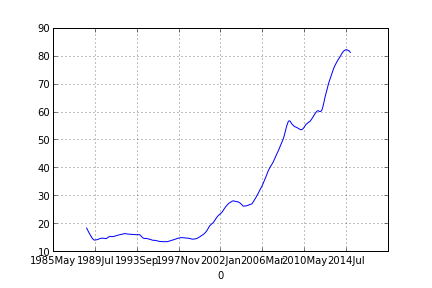
\includegraphics[height=6cm]{corr_01.png}


\begin{minted}[fontsize=\footnotesize]{python}
print len(list(pd.rolling_mean(df[1],80).dropna()))
\end{minted}

\begin{verbatim}
276
\end{verbatim}

\begin{minted}[fontsize=\footnotesize]{python}
import pandas as pd
import datetime
from dateutil.parser import parse
price = pd.read_csv('oilprice.csv',header=None,index_col=0)
prod = pd.read_csv('world.csv',parse_dates=True,index_col=0,sep=' ')
price.index = map(lambda x: datetime.datetime.strptime(x,'%Y%b'), price.index)
prod['price'] = price
print prod.price.corr(prod.oil)
\end{minted}

\begin{verbatim}
0.812066270665
\end{verbatim}

\begin{minted}[fontsize=\footnotesize]{python}
prod.plot()
plt.savefig('corr_02.png')
\end{minted}

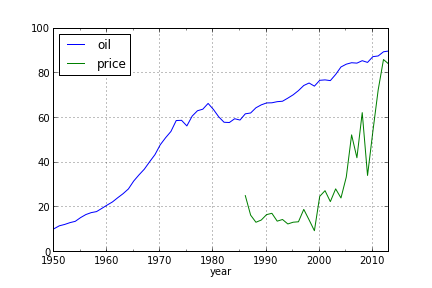
\includegraphics[height=6cm]{corr_02.png}

\begin{minted}[fontsize=\footnotesize]{python}
import pandas as pd
df = pd.read_csv('burgersold.csv',sep=' ',header=None,index_col=0,names=['sold'])
df['price'] = pd.read_csv('burgerprice.csv',sep=' ',header=None,index_col=0)
df['price'] = bs['price'].interpolate()
print df.sold.corr(df.price)
print df[:10]
\end{minted}

\begin{verbatim}
0.912052062441
      sold  price
1969  2142    NaN
1970  2142    NaN
1971  2142    NaN
1972  2142    NaN
1973  2142    NaN
1974  2142    NaN
1975  2142  0.300
1976  2142  0.325
1977  3750  0.350
1978  3750  0.375
\end{verbatim}

http://the-american-catholic.com/2014/11/21/wages-and-hamburgers-a-pricing-history/

\begin{minted}[fontsize=\footnotesize]{python}
df['price'].plot()
plt.savefig('corr_03.png')
\end{minted}

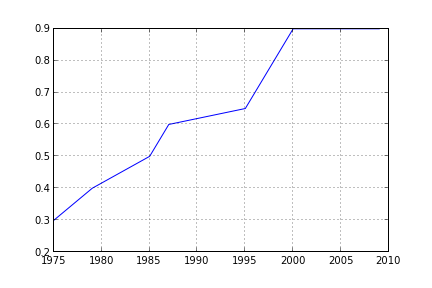
\includegraphics[height=6cm]{corr_03.png}


\begin{minted}[fontsize=\footnotesize]{python}
df['sold'].plot()
plt.savefig('corr_04.png')
\end{minted}

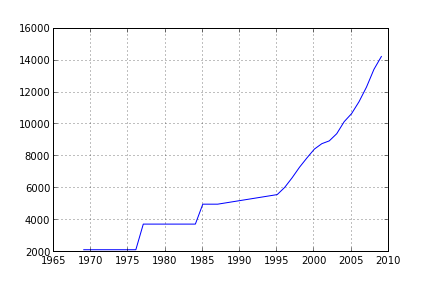
\includegraphics[height=6cm]{corr_04.png}






\begin{minted}[fontsize=\footnotesize]{python}
p = 0.56; tmp = 1.96*np.sqrt((1/42.)*p*(1-p)); print p-tmp, p+tmp
\end{minted}

\begin{verbatim}
0.409875429504 0.710124570496
\end{verbatim}





\end{document}
